\usetheme{Bergen}  %% Themenwahl
 
\usepackage[utf8]{inputenc}
\usepackage{graphicx}
\usepackage{hyperref}
\usepackage[absolute,overlay]{textpos}


\title{Erlang - Verteilte Systeme eine neue Erfindung?}
\author{Jannis Hübl - @HblHuebl}
\date{\today}
 
\begin{document}
\maketitle

\mode<article>
   \newpage
\mode*

\frame{\tableofcontents[currentsection]}
 
\mode<article>
   \newpage
\mode*

\section{Wie ich zu Erlang gefunden habe..}
\subsection{Die Idee}
\begin{frame} %%Eine Folie
  \frametitle{Die Idee} %%Folientitel
  \begin{itemize} %%Definition
     \item<1-> Eine App schreiben. (Done)
     \item<2-> Eine App schreiben deren Daten auf einem eigenen Server gespeichert werden. (In Progress)
     \item<3-> Ein eigenes P2P-Netz bauen. (Planed) 
     \item<4-> Einen Server schreiben der eine bilatarale Kommunikation zulässt. (In Progress)
     \item<5-> Eigene Pushnachrichten verschicken ohne Google. (Done)
     \item<6-> Die Lösung: RabbitMQ.
  \end{itemize}
\end{frame}
\note{test notize}

\subsection{RabbitMQ}
\begin{frame} %%Eine Folie
  \frametitle{RabbitMQ} %%Folientitel
  \begin{itemize} %%Definition
    \item Messagebroker
    \item Realiesierung eines Pushservice
    \item Implementierung von AMQP 
    \item Programmiersprache: Erlang
  \end{itemize}
  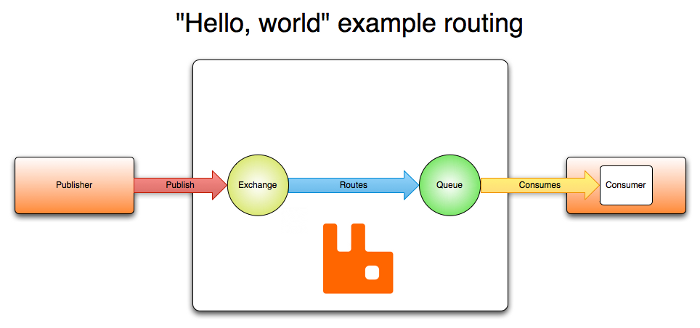
\includegraphics[width=250px]{img/example-routing}
\end{frame}


\begin{frame} %%Eine Folie
  \frametitle{Was ist Erlang?} %%Folientitel
  \pause
  \begin{itemize}[<+->] %%Definition
    \item Programmiersprache
  \end{itemize}
\end{frame}

\begin{frame} %%Eine Folie
  \frametitle{Für was Erlang?} %%Folientitel
  \pause
  \begin{itemize}[<+->] %%Definition
    \item massively scalable
    \item soft real-time systems
    \item high availability
  \end{itemize}
\end{frame}

\section{Konzepte in Erlang}
\begin{frame} %%Eine Folie
  \frametitle{Konzepte in Erlang} %%Folientitel
  \begin{itemize} %%Definition
    \item Nebenläufigkeit (nicht Parallelisierung!!)
    \item Verteilte Systeme
    \item Fehlertoleranz
  \end{itemize}
\end{frame}

\subsection{Nebenläufigkeit}
\begin{frame} %%Eine Folie
  \frametitle{Aktoren Model} %%Folientitel
  \begin{itemize} %%Definition
    \item Gefängnisinsassen in ihren Zellen
    \item Kommunizieren ausschießlich über Briefe
  \end{itemize}
  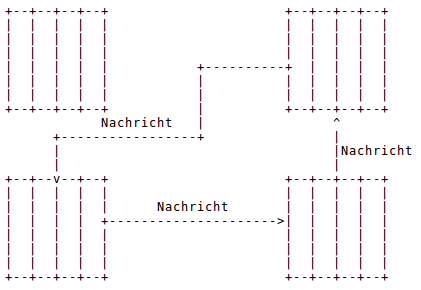
\includegraphics[width=250px]{img/actoren}
\end{frame}

\subsection{Verteilte Systeme}
\begin{frame} %%Eine Folie
  \frametitle{Verteilte Systeme} %%Folientitel
    Siehe 6. Semester bei Florian Sperber
    \begin{center}
       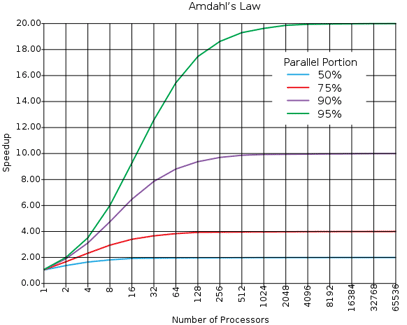
\includegraphics[width=250px]{img/amdahl}
    \end{center}
\end{frame}

\subsection{Fehlertoleranz}
\begin{frame} %%Eine Folie
  \frametitle{Fehlertoleranz} %%Folientitel
  \begin{itemize} %%Definition
    \item Let it crash!!
    \item Durch Aktoren stützen nur einzelne Teile ab.
    \item Andere Programmteile sollen den Fehler abhandeln.
  \end{itemize}
\end{frame}

\section{Development enviroment}
\begin{frame} %%Eine Folie
  \frametitle{Development enviroment} %%Folientitel
  \begin{itemize} %%Definition
    \item Eigene VM (Unterstützung für JVM)
    \item Development tools (compiler, debugger, profiler, test framework)
    \item Open Telecom Platform (OTP) Framework
    \item Web server
    \item Parser Generator
    \item Mnesia Datenbank
    \item Hot code loading
  \end{itemize}
\end{frame}

\subsection{Open Telecom Platform (OTP) Framework}
\begin{frame} %%Eine Folie
  \frametitle{Open Telecom Platform (OTP) Framework} %%Folientitel
  \begin{Definition}
    Sammlung von Designpattern (Funktional!!)
  \end{Definition}
  \begin{itemize} %%Definition
    \item FSM (Entlicher Automat)
    \item Server (Clients sind andere Prozesse)
    \item Supervisor (Beobachten, Kontrollieren andere Prozesse)
  \end{itemize}
\end{frame}

\begin{frame} %%Eine Folie
  \frametitle{Was Lernen wir daraus?} %%Folientitel
  \begin{center}
     abstrahieren, abstrahieren, abstrahieren!!
     \newline
     - Erlang erlaubt es also benutzt es
   \end{center}
\end{frame}


\subsection{Mnesia}
\begin{frame} %%Eine Folie
  \frametitle{Mnesia} %%Folientitel
  \begin{Definition}
    In Memory Database
  \end{Definition}
  \begin{itemize} %%Definition
    \item Wird über alle Erlangnodes synchronisiert
    \item Erlaubt Zugriff auf selbe Daten von verschiedenen Aktoren
    \item Recht kompliziert
  \end{itemize}
\end{frame}

\subsection{Hot code loading}
\begin{frame} %%Eine Folie
  \frametitle{Hot code loading} %%Folientitel
  \begin{Definition}
    Programmcode während des Betriebs ändern
  \end{Definition}
  \begin{itemize} %%Definition
    \item VM kann zwei Codeversionen aufnehmen
    \item Neuer Aufrufe des Codeteils -> Neuer Code wird geladen
    \item Probleme:
      \begin{itemize}
        \item Prozess steht still.
        \item "Objekte" müssen geändert werden.
      \end{itemize}
    \item Lösungen:
      \begin{itemize}
        \item Let it fail.
        \item Methoden um Programmstatus zu ändern.
      \end{itemize}
  \end{itemize}
\end{frame}

\begin{frame} %%Eine Folie
  \frametitle{Was lernen wir daraus?} %%Folientitel
  Mach es nicht wenn du es nich umbedingt brauchst!!
\end{frame}

\section{Was ist den nun Erlang?}
\begin{frame} %%Eine Folie
  \frametitle{Was ist den nun Erlang?} %%Folientitel
  \begin{itemize} %%Definition
    \item Erlang bietet die Möglichkeit kranken Scheiss zu machen.
    \item Erlang ist keine Patentlösung für alles.
    \item Erlang ist keine Patentlösung für verteilte Systeme.
    \item Erlang ist keine Patentlösung für Nebenläufigkeit.
    \item Erlang bietet die Möglichkeiten dazu.
  \end{itemize}
\end{frame}

\section{Erlang History}
\begin{frame} %%Eine Folie
  \frametitle{Erlang History} %%Folientitel
  \begin{itemize} %%Definition
    \item Kommt aus der Telekomunikationsbranche (Ericsson)
    \item Erste Implementierung in Prolog
    \item Von ca. 1990 (fyi: ~24 Jahre)
  \end{itemize}
\end{frame}

\section{Literatur}
\begin{frame} %%Eine Folie
  \frametitle{Literatur} %%Folientitel
  \begin{itemize} %%Definition
    \item Learn you some Erlang for Greate Good! - A Beginner's Guide
    \item \url{http://learnyousomeerlang.com/}
  \end{itemize}
  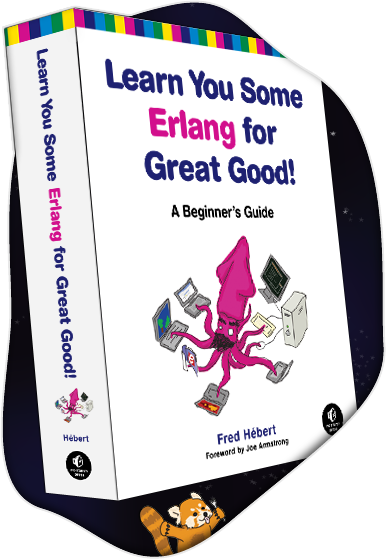
\includegraphics[height=200px]{img/splash-book}
\end{frame}

\section{Coole Software}
\begin{frame} %%Eine Folie
  \frametitle{Coole Software} %%Folientitel
  \begin{itemize} %%Definition
    \item RabbitMQ
    \item CouchDB (auch für IOS, Android)
    \item SimpelDB (Amazon)
    \item Farwest (front-end)
    \item eJabberd
    \item Chef seit v11 
    \item Game-Server
    \item Trading (zB. Goldman Sachs)
  \end{itemize}
\end{frame}

\mode <presentation>
\begin{frame} %%Eine Folie
  \frametitle{Fork me on Github} %%Folientitel
   \begin{textblock*}{3cm}(10cm,0cm) % {block width} (coords)
   
\includegraphics[width=3cm]{img/forkme}
   \end{textblock*}
  \begin{itemize} %%Definition
    \item Präsentation: \url{https://github.com/jannishuebl/erlang-pre}
    \item P2Pf:         \url{https://github.com/p2pf}
  \end{itemize}
\end{frame}
\mode*

\mode <article>
\section{Fork me on Github}
  \begin{itemize} %%Definition
    \item Präsentation: \url{https://github.com/jannishuebl/erlang-pre}
    \item P2Pf:         \url{https://github.com/p2pf}
  \end{itemize}
\mode*

\end{document}
